\documentclass{beamer}

\usepackage{graphicx}

\begin{document}
 %=============================================================== %
\begin{frame}
	
\begin{figure}
\centering
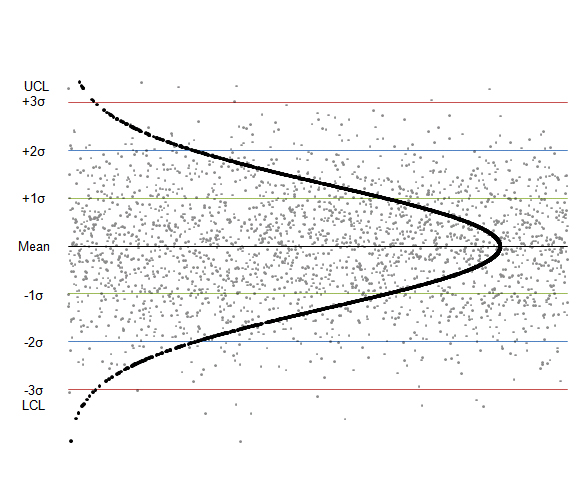
\includegraphics[width=1.0\linewidth]{images/ControlChart}
\end{figure}
	
\end{frame}
\begin{frame}
	
	\begin{figure}
		\centering
		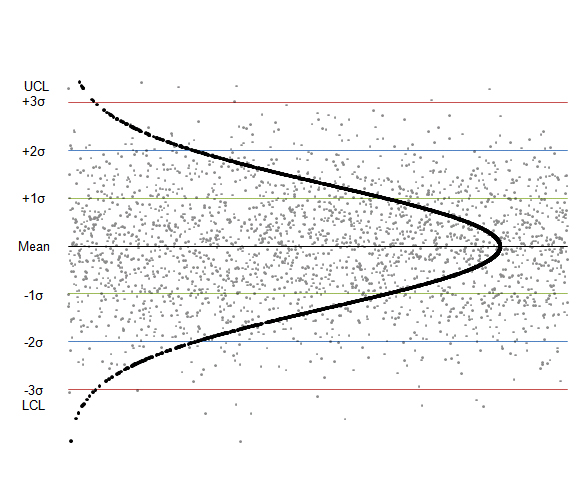
\includegraphics[width=1.0\linewidth]{images/ControlChart}
	\end{figure}
	
\end{frame}
\begin{frame}
	
	\begin{figure}
		\centering
		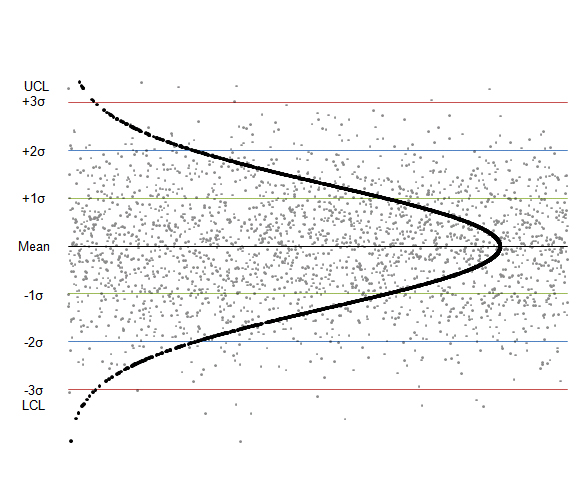
\includegraphics[width=1.0\linewidth]{images/ControlChart}
	\end{figure}
	
\end{frame}
\begin{frame}
	
	\begin{figure}
		\centering
		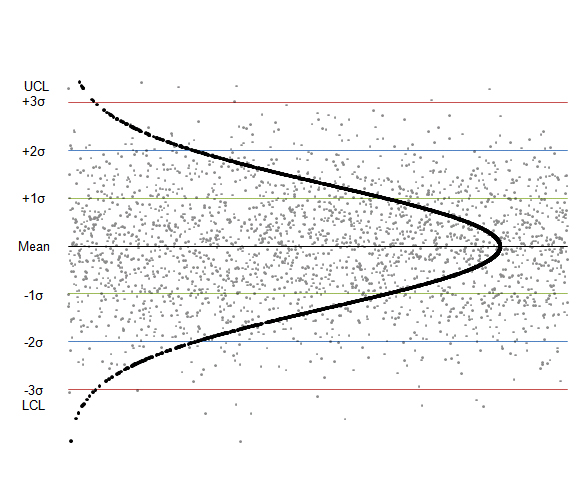
\includegraphics[width=1.0\linewidth]{images/ControlChart}
	\end{figure}
	
\end{frame}
%============================================================= %
\begin{frame}
\frametitle{Control Limits}
\begin{figure}
\centering
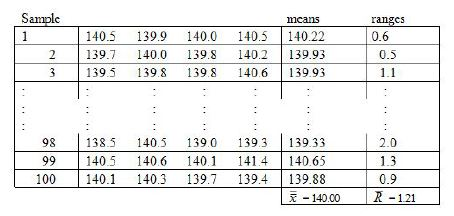
\includegraphics[width=1.1\linewidth]{C:/Users/Kevin/Documents/GitHub/SPCWithR/ControlLimits1}
\end{figure}

\end{frame}
%============================================================= %
\begin{frame}
	\frametitle{Control Limits}
	\begin{figure}
		\centering
		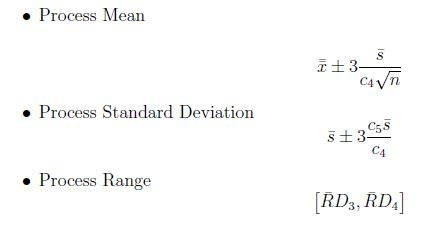
\includegraphics[width=1.1\linewidth]{C:/Users/Kevin/Documents/GitHub/SPCWithR/ControlLimits2}
	\end{figure}
	
\end{frame}
%============================================================= %
\begin{frame}
	\frametitle{Control Limits}
	\begin{figure}
		\centering
		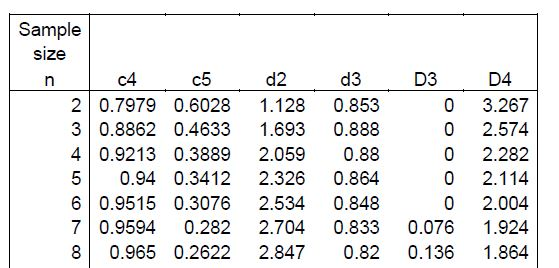
\includegraphics[width=1.1\linewidth]{C:/Users/Kevin/Documents/GitHub/SPCWithR/ControlLimits3}
	\end{figure}
	
\end{frame}

\begin{frame}
	\frametitle{Control Limits}
	
\end{frame}

\begin{frame}
	\frametitle{Control Limits}
	
\end{frame}

\begin{frame}
	\frametitle{Control Limits}
	
\end{frame}

\begin{frame}
	\frametitle{Control Limits}
	
\end{frame}
%============================================================= %
\end{document}
